\section{Spørsmål Runde 1 }
%Jeg har funnet et program kalt \textbf{Engauge Digitizer} til å lese av grafene. Sliter litt med 
%at den ikke identifiserer alle kurvene og sliter med overlappende biter.
%\newline
%\begin{wrapfigure}{r}{0.6\textwidth} %Requires the package wrapfigure
  %\begin{center}
    %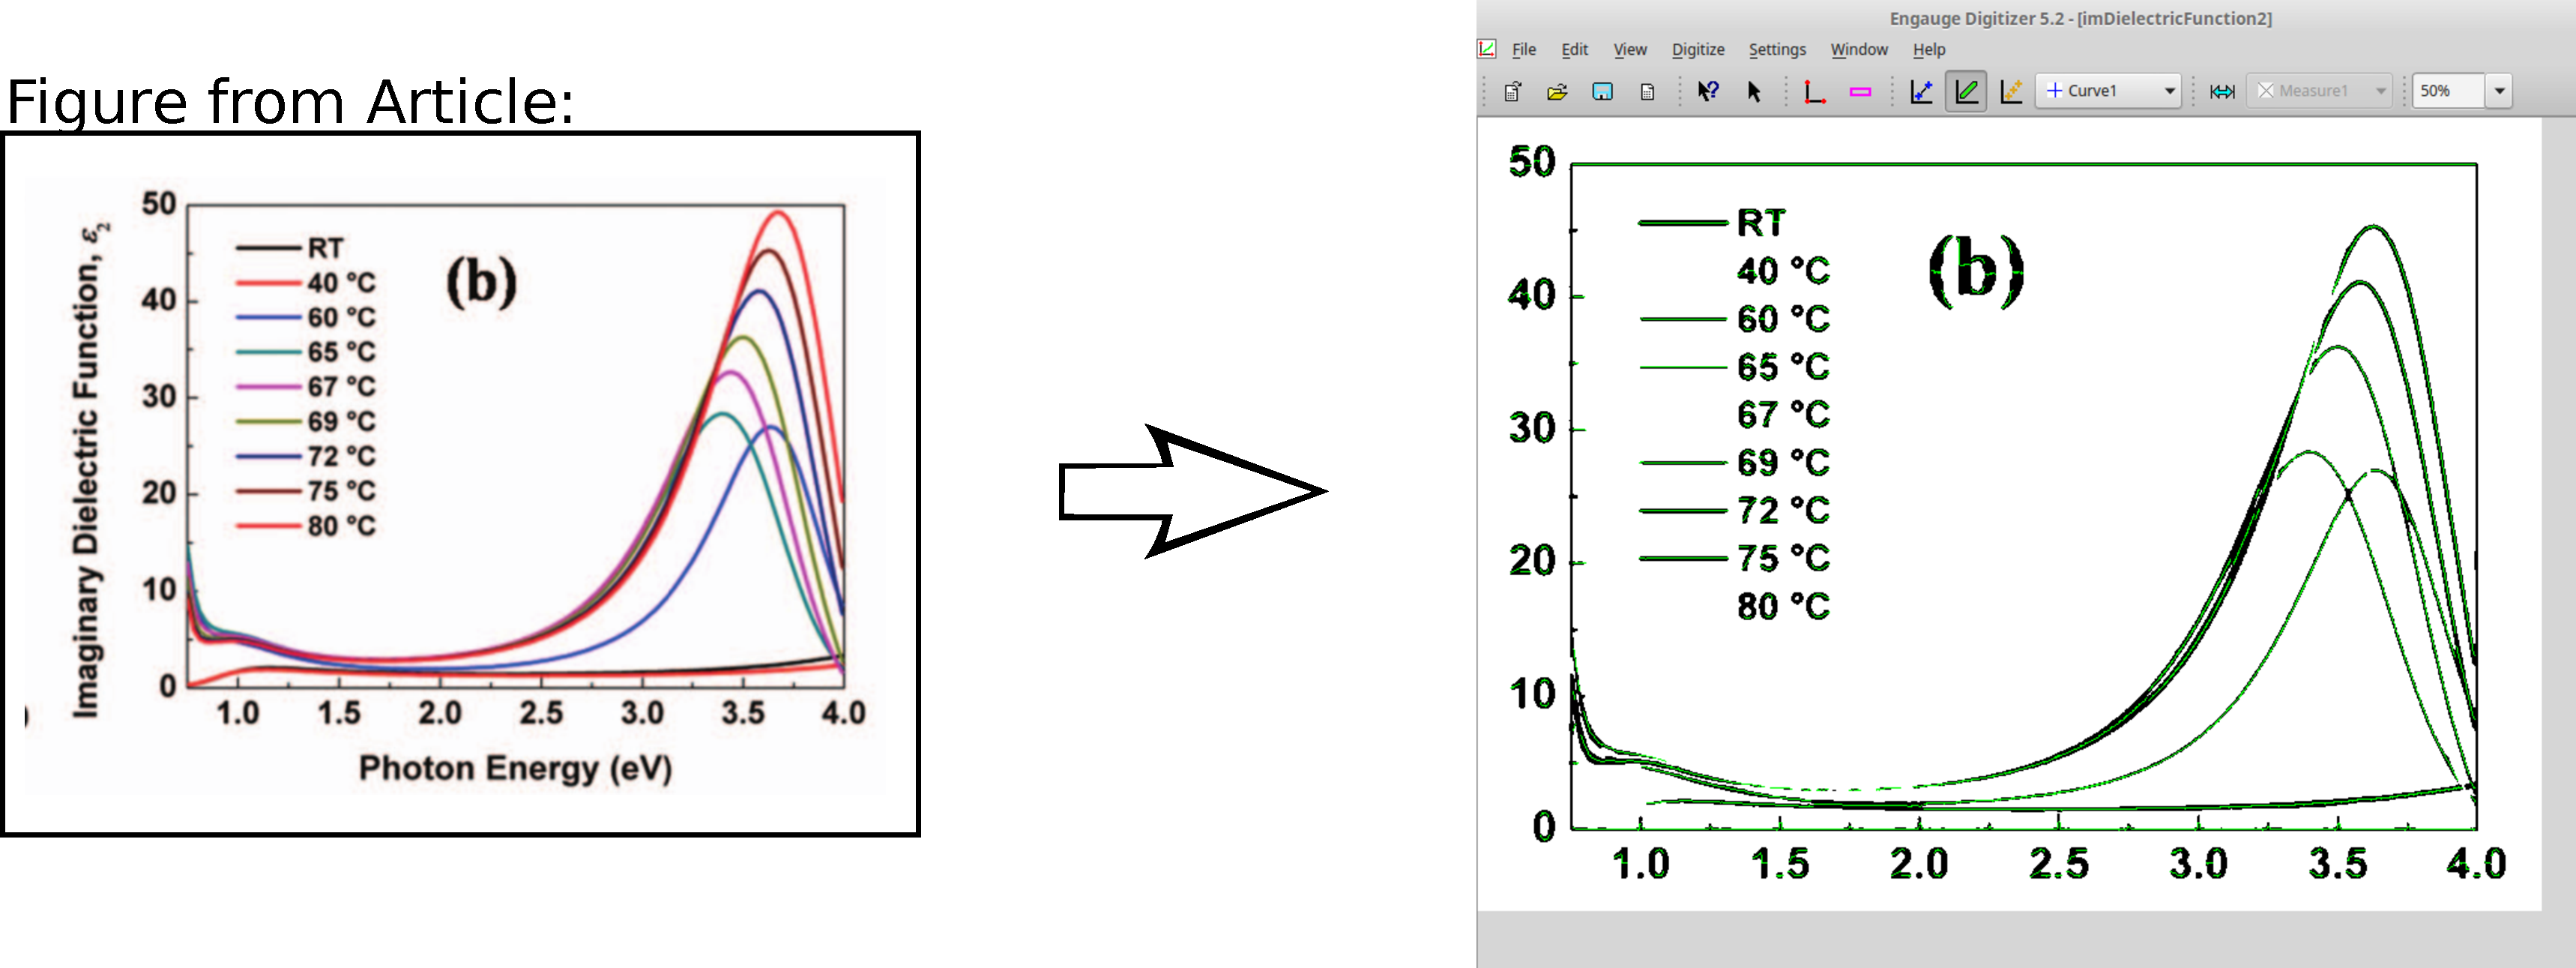
\includegraphics[width=0.58\textwidth]{engaugeExample.pdf}
  %\end{center}
%\end{wrapfigure}
Jeg prøver å forstå mer detaljert hvordan jeg skal få lest inn dataen til GranFilm programmet.
Formatet til ''.nk''-filene i \texttt{GranFilm/Sopra/DataBase} ser slik ut (her mgo.nk):
\begin{lstlisting}[style=FormattedNumber,frame=none]
   1		0.65			10		400    
        1.70969699     0.00000011
        1.71065583     0.00000011
        1.71239613     0.00000011
\end{lstlisting}
og ser ut til å ha reell og imaginær refraksjonsindeks forholdsvis på kolonne 1 og 2. I tillegg virker det
som om rad èn består av de 4 verdiene: 
\begin{itemize}
   \item unit (om refraksjonsindeksen er funksjon av energi (eV) 
eller bølgelengde); 
\item x startverdi (energi/bølgelengde); 
\item x sluttverdi
\item antall datapunkter.
\end{itemize}
Basert på dette, i tillegg til modulen fra source-koden til GranFilm gitt nedenfor, virker det
som om reell og imaginær verdi er gitt for samme x-verdi (energi/bølgelengde), der x-verdiene 
har konstant steglengde. (For eksempel: for mgo.nk filen ville vi hatt $d\!x = \frac{10-0.65}{400-1}$).
\\
\\
Jeg har funnet et program som lar meg hente ut dataen fra grafer i artikklene. 
Prolemet er at dataen for reell og imaginær refraksjonsindeks 
er for forskjellige x-verdier, der x-verdiene ikke har
konstant steglengde.\\
\\
\textbf{Spørsmålene er derfor:} 
\begin{enumerate}
   \item Er det riktig det jeg har forstått ovenfor? 
   \item Trenger jeg skrive om inputfilene (filene med thermochrom-dataen) 
      slik at reell og imaginær verdi (forholdsvis $n$,$k$)
      svarer til samme x-verdi, der x-verdiene ligger med avstand $d\!x$ i fra hverandre?\\
      (Jeg tenkte å kanskje skrive en funksjon som tar inn to filer, colonner og ''unit''-verdi, 
      leser inn $n$ og $k$ dataen fra filene, intrapolerer for felles, nye x-verdier og skriver til 
      en ny fil.)
   \item Videre: noen grafer er gitt ved permittivitet $\varepsilon$, istedenfor refraksjonsindex \textbf{n}.
      Da er det vel bare å regne om ved bruk av imaginær permittivitet? Jeg fant noen formlet og lurte på 
      om dette er riktig: fant at 
      \begin{align*}
         \boldsymbol{\varepsilon} =
            \frac{c^2 \varepsilon_0}{\omega^2 \frac{\mu}{mu_0}} \Bigg( k^2 - \frac{\alpha ^2}{4}\Bigg)  
            + i\Bigg( \frac{c^2 \varepsilon_0}{\omega^2 \frac{\mu}{\mu_0}} k \alpha \Bigg)
      \end{align*}
      ($k$ er hær bølgetallet), hvor 
      \begin{align*}
         &\boldsymbol{n} = k - i\frac{\alpha}{2}, & \boldsymbol{n} = \frac{c}{\omega} \boldsymbol{k}^*.
      \end{align*}
      Bruker at $\mu = \mu_0$ og får
      \begin{align*}
         &\text{Re}(n) = \frac{\text{Im}(\varepsilon)}{2 \varepsilon_0} \\
         &\text{Im}(n) = \sqrt{\frac{\text{Re}(\varepsilon)}{\varepsilon_0} - 
         \Bigg( \frac{\text{Im}(\varepsilon)}{2 \varepsilon_0} \Bigg) ^2}.
      \end{align*}
\end{enumerate}

Til slutt vil jeg bare si at framgangen går sakte, og begynner å bli litt stresset mtp tiden. Lurte
på hvor mye du hadde forestilt deg at jeg burde få til? Foreløpig, har jeg klart å lese ut 
VO$_2$-dataen fra de fire artiklene du sendte meg. Dataene trenger trolig mer arbeid før de mates inn
i GranFilm som beskrevet ovenfor. Der ligger VO$_2$ data for 10-12 forskjellige temperaturer.


%I kildekoden til \texttt{GranFilm} fant jeg \texttt{dielectric\_function\_module.f90}:
%\begin{lstlisting}[style=FormattedNumber,frame=none, language=FORTRAN]
    %Read(unit=ifile,fmt=*) unit,x1,x2,lines
    %dx = (x2 - x1)/(lines-1)

    %Allocate( x(lines), y(lines) )
    %Select Case (unit)
    %Case(1)
       %! Unit = Electron Volt (eV)
       %Do i=1,lines 
          %Read(unit=ifile,fmt=*) tmp(1), tmp(2)
          %x(i) = x1 + (i-1)*dx
          %y(i) = tmp(1)+imu*tmp(2)
       %Enddo
    %Case(2)
       %! Unit = WaveLength (microm)
       %Do i=lines,1,-1 
          %Read(unit=ifile,fmt=*) tmp(1), tmp(2)
          %x(i) = x1 + (lines-i)*dx
          %y(i) = tmp(1)+imu*tmp(2)
       %Enddo
       %x(:) = 1.243\_wp/x(:) ! Conversion microm-->eV
    %End Select

    %Close(unit=ifile)
%\end{lstlisting}
%først leses første linje av \texttt{'.nk'}-filen:
%som gir \texttt{unit} (som er hva?), start energi/bølgelengde, slutt energi/bølgelengde og til slutt 
%antall datapunkter. Når du nå regner ut \texttt{x} og \texttt{y} virker det som om du antar at
%n,k-verdiene er gitt from samme energi(eV) eller bølgelengde. I tillegg virker det som at datapunktene
%må være separert med konstant steglengde $dx$. Men, i mine avleste data
%er ikke dette tilfellet: dataen er gitt for ulike verdier og steglengden varierer: 
%\begin{lstlisting}[style=FormattedNumber,frame=none]
   %//#! Fra fil reIndexOfRefractionVO2.csv,
   %x,n06,n13
   %3.40909e-07,1.96538,1.01971
   %3.45455e-07,2.12453,1.15231
   %3.61364e-07,2.68154,1.61639
   %.           .       .
   %.           .       .
%\end{lstlisting}
%\begin{lstlisting}[style=FormattedNumber,frame=none]
   %//#! Fra fil imIndexOfRefractionVO2.csv
   %x,k06,k13
   %3.41541e-07,1.44393,0.928804
   %3.42121e-07,1.43807,0.933948
   %3.51121e-07,1.34701,1.01382
   %.           .       .
   %.           .       .
%\end{lstlisting}
%Må jeg passe på at input-data-filen er slik som jeg har tolket ovenfor, altså:
%to kolonner (første med reel refraksjonsindex og andre med imaginer refraksjonsindex)
%der verdiene i en gitt rad er gitt for samme x-verdi (energi/bølgelengde)?\\
%\\
%Hele koden for funksjonen er hær:
I kildekoden til \texttt{GranFilm} \: fant jeg modulen \: \texttt{dielectric\_function\_module.f90}.
Forstår det slik at 
\begin{lstlisting}[style=FormattedNumber, language=FORTRAN, frame=none]
    Function Locate(xx,x)
\end{lstlisting}
finner indeksen i xx til elementet som ligger nærmest verdien x? Tenkte å kunne bruke
funksjonen eller skrive den om, og bruke den i intrapolering om jeg må skrive om input-filene.
\begin{lstlisting}[style=FormattedNumber, language=FORTRAN]
  !------------------------------------------------------------!
  Subroutine Get_Dielectric_Function(energy,epsilon,material,path)
  !Subroutine dielectric_constants(energy,epsilon,material,path)
  !------------------------------------------------------------!
    Use SFL_Logical_Units,       only : SFL_Get_Free_Unit
    Use Error_Module,            only : Error_Failure
    Implicit None
    Real(wp)                          :: energy(:)
    complex(wp )                      :: Epsilon(:)
    Character(len=*)                  :: material
    Character(len=*)                  :: path
    ! --- Local
    Character(len=*), parameter       :: routine = "Get_Dielectric_Function"
    !complex(wp ),Parameter            :: im=(0._wp,1._wp)
    Character(len=250)                :: filename, str
    Logical                           :: exi
    integer                           :: lines,start,i, ifile
    Real(wp),     Allocatable         :: x(:)
    complex(wp ), Allocatable         :: y(:)
    Real(wp)                          :: tmp(2),x1,x2,dx
    integer                           :: unit, istat
    complex(wp )                      :: slope
    

    ! Opens the relevant data file for the given material
    ! Notice that the data-files contains the values for the 
    ! index of refraction, n,k extacted from the data base of
    ! SOPRA.
    ! Therefore "epsilon = epsilon**2" at the bottom of this routine    
    filename = Trim(Adjustl(path))//'/'//Trim(Adjustl(material))//'.nk'
    Inquire(file=Trim(Adjustl(filename)),exist = exi)
    If( .NOT. exi ) Then
       write(str,*) trim(adjustl(filename))
       str = "File = " // trim(adjustl(str)) // " non existing" 
       Call Error_Failure(routine, trim(adjustl(str)) )
    Endif
    call SFL_Get_Free_Unit( ifile )
    Open(unit=ifile,file=filename,status='old')
    Read(unit=ifile,fmt=*) unit,x1,x2,lines
    dx = (x2 - x1)/(lines-1)

    Allocate( x(lines), y(lines) )
    Select Case (unit)
    Case(1)
       ! Unit = Electron Volt (eV)
       Do i=1,lines 
          Read(unit=ifile,fmt=*) tmp(1), tmp(2)
          x(i) = x1 + (i-1)*dx
          y(i) = tmp(1)+imu*tmp(2)
       Enddo
    Case(2)
       ! Unit = WaveLength (microm)
       Do i=lines,1,-1 
          Read(unit=ifile,fmt=*) tmp(1), tmp(2)
          x(i) = x1 + (lines-i)*dx
          y(i) = tmp(1)+imu*tmp(2)
       Enddo
       x(:) = 1.243_wp/x(:) ! Conversion microm-->eV
    End Select

    Close(unit=ifile)

    ! --- Do the interpolation
    Do i=1,Size(energy,1)
       start=locate(x(:),energy(i))
       If((start==0).Or.(start==lines)) Then
          write(str,"('Energy not in range : ',f5.2,' for i=',i3)") energy(i),i
          call Error_Failure( routine, trim(adjustl(str)))
       Endif
       ! Linear interpolation
       slope = (y(start+1)-y(start))/(x(start+1)-x(start))
       Epsilon(i) = y(start) + slope*(energy(i)-x(start))
       !            Write(unit=67,*) energy(i),Real(epsilon(i)),Aimag(epsilon(i))
    Enddo
    
    ! --- Calculates the dielectric constant (from the refraction index)
    epsilon = epsilon**2
    Deallocate(x,y,stat=istat)

  contains
    
    Function Locate(xx,x)
      Implicit None
      Real(wp), Dimension(:), Intent(In)  :: xx
      Real(wp), Intent(In)                :: x
      Integer                             :: locate
      Integer                             :: n,jl,jm,ju
      Logical                             :: ascnd
      
      n=Size(xx)
      ascnd = (xx(n) >= xx(1))
      jl=0
      ju=n+1
      Do
         If(ju-jl <= 1) exit
         jm=(ju+jl)/2
         If(ascnd .eqv. (x >= xx(jm))) Then
            jl=jm
         Else
            ju=jm
         Endif
      Enddo
      If(x == xx(1)) Then
         locate=1
      Else If(x == xx(n)) Then
         locate=n-1
      Else
         locate=jl
      Endif
      
    End Function Locate
    

  End Subroutine Get_Dielectric_Function
  !-------------------------------------!
\end{lstlisting}

